\section{Simmetria \PT\ e \CPT}
\begin{frame}{Operatori \PT-invarianti}
    Diciamo che un operatore è \hPT-invariante se
    $$\PTtransform{\hA} = \hA\mycomma$$
    o analogamente
    $$\comm*{\hPT}{\hA}\! = 0\myperiod$$
    \pause
    Se $\ket{\psi}$ è un autostato \emph{simultaneo} di \hA\ e \hPT, l'autovalore $\lambda$ di \hA\ associato a $\ket{\psi}$ è \emph{reale}, infatti
    \begin{align*} 
        \hPT\pqty*{\hA\!\ket{\psi}}\! = \hPT\pqty{\lambda\!\ket{\psi}}
        \quad&\iff\quad
        \pause
        \hA\hPT\!\ket{\psi} = \lambda^*\hPT\!\ket{\psi} \\
        \pause
        \hA\!\ket{\psi} = \lambda^*\!\ket{\psi}
        \quad&\iff\quad
        \lambda\!\ket{\psi} = \lambda^*\!\ket{\psi}
    \end{align*}
\end{frame}

\begin{frame}
    Domanda:
    \begin{center}
        {\it Esiste una classe più generale di operatori con autovalori reali?}
    \end{center}
    Risposta:
    \pause
    \begin{center}
        {\it Sì e no, perché non tutti gli operatori Hermitiani sono \emph{anche} \PT-invarianti, ma esistono operatori \emph{non Hermitiani} che hanno autovalori reali.}
    \end{center}
    \pause
    \begin{figure}
        \centering
        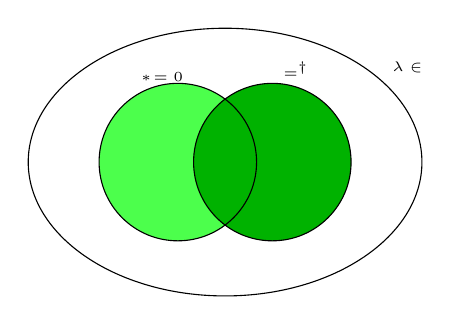
\begin{tikzpicture}
            \fill[color=green!70!white] (-0.6,0) circle (1);
            \fill[color=green!70!black] (0.6,0) circle (1);
            \draw (-0.6,0) circle (1);
            \draw (+0.6,0) circle (1);
            \draw (0,0) ellipse (2.5 and 1.7);
            \node[anchor=south] at (0.9,0.95) {\tiny{$\hH = \hH^\dag$}};
            \node[anchor=south, align=center] at (-0.8,0.9) {\tiny{$\comm*{\hPT}{\hH}\! = 0$}};
            \node[anchor=west, align=center] at (2,1.2) {\tiny{$\lambda\in\bbR$}};
        \end{tikzpicture}
    \end{figure}
\end{frame}

\begin{frame}{Simmetria \PT}
    Diciamo che un sistema fisico \emph{non rompe la Simmetria \PT} se
    \begin{enumerate}[label=\mybullet]
        \pause
        \item L'Hamiltoniana \hH\ commuta con \hPT;
        \pause
        \item Gli autostati di \hH\ sono simultaneamente autostati di \hPT.
    \end{enumerate}
    \pause
    In questo caso lo spettro di \hH, ovvero le possibili misure di energia, sono reali.
\end{frame}

\begin{frame}
    Una nuova domanda:
    \begin{center}
        {\it Possiamo costruire una teoria quantistica a partire da Hamiltoniane \PT-invarianti?}
    \end{center}
\end{frame}

\begin{frame}{Ci siamo persi qualcosa...}
    Quali sono le proprietà fondamentali di cui una teoria quantistica non può fare a meno?
    \begin{enumerate}
        \pause
        \item[\ding{51}] Le misure devono essere numeri reali;
    \end{enumerate}
    \pause
    inoltre, nello spazio di Hilbert deve essere definito un prodotto interno tale che
    \begin{enumerate}
        \pause
        \item[\ding{55}] Gli autospazi siano ortogonali;
        \pause
        \item[\ding{55}] La probabilità si conservi;
    \end{enumerate}
    \pause
    Senza farci caso abbiamo perso le ultime due proprietà.
\end{frame}

\begin{frame}{Prodotto \PT}
    Il prodotto scalare Hermitiano tra due stati $\ket{\psi},\ket{\phi}$ si ottiene moltiplicando un vettore per l'Hermitiano coniugato dell'altro,
    $$
        \braket{\phi}{\psi} = \int\nolimits_{\bbR^3}\phi^*\pqty{\vb{r}}\psi\pqty{\vb{r}} \dd[3]{\vb{r}}
    $$
    \pause
    Rispetto a \emph{questo} prodotto scalare, gli autostati di un'Hamiltoniana \PT-invariante, ma \emph{non Hermitiana}, non sono ortogonali.
\end{frame}

\begin{frame}{Prodotto \PT}
    Possiamo introdurre un prodotto \PT, che al posto della coniugazione Hermitiana fa uso della trasformazione \hPT :
    \pause
    $$
        \braket{\phi}{\psi}_{\PT} = \int\nolimits_{\bbR^3} \phi^{\PT}\!\pqty{\vb{r}}\pause\psi\pqty{\vb{r}} \dd[3]{\vb{r}}
        \mycomma
    $$
    \pause
    dove $\phi^{\PT}\!\pqty{\vb{r}} = \phi^*\pqty{-\vb{r}}$, \pause coerente con:
    \begin{enumerate}[label=\mybullet]
        \item $\func{\hP}{\vb{r}}{-\vb{r}}$
        \item $\func{\hT}{\lambda}{\lambda^*}$
    \end{enumerate}
    \pause
    Rispetto a questo prodotto, gli autostati di \hH\ sono di nuovo ortogonali ma questo prodotto non è definito positivo.

    \pause
    Si dimostra inoltre che
    \begin{equation*}
        \norm{\ket{\phi_n}}_{\PT}^2 = \braket{\phi_n}{\phi_n}_{\PT} = \pqty{-1}^n
        \myperiod
    \end{equation*}
\end{frame}

\begin{frame}{L'operatore \hC}
    Per recuperare la definita positività bisogna costruire un prodotto \CPT\ dove \hC\ rappresenta un nuovo operatore lineare tale che:
    \begin{enumerate}[label=\mybullet]
        \pause
        \item $\comm*{\hC}{\hH}\! = 0$;
        \pause
        \item $\comm*{\hC}{\hPT}\! = 0$;
        \pause
        \item $\hC^2 = \hidM$;
    \end{enumerate}
    \pause
    L'operatore può essere costruito nella base della della posizione come
    \begin{equation*}
        \mel*{\vb{r}}{\hC}{\vb{r'}} = \sum\nolimits_n \phi_n\pqty{\vb{r}}\phi_n\pqty*{\vb{r}'}
        \myperiod
    \end{equation*}
    \pause
    Si può inoltre trovare una funzione $Q$ tale che
    \begin{equation*}
        \hC = \myexp{Q\pqty{\hvr,\hvp}}\hP
        \myperiod
    \end{equation*}
\end{frame}

\begin{frame}{Operatore \hC}
    Svolgendo un po' di calcoli si trova:
    \begin{align*}
        \mel{\vb{r}}{\hC}{\phi_n}
        &= \int\nolimits_{\bbR^3} \mel*{\vb{r}}{\hC}{\vb{r'}}\!\!\!\braket*{\vb{r}'}{\phi_n} \dd[3]{\vb{r}'} \\
        &= \sum\nolimits_m \phi_m\pqty{\vb{r}} \int\nolimits_{\bbR^3} \phi_m\pqty*{\vb{r}'} \phi_n\pqty*{\vb{r}'} \dd[3]{\vb{r}'} \\
        &= \sum\nolimits_m \phi_m\pqty{\vb{r}} \pqty{-1}^m \tensor{\delta}{_m_n} \\
        &= \pqty{-1}^n \phi_n\pqty{\vb{r}}\mycomma
    \end{align*}
    ovvero
    \begin{equation*}
        \hC\!\ket{\phi_n} = \pqty{-1}^n\!\ket{\phi_n}
        \myperiod
    \end{equation*}
\end{frame}

\begin{frame}{Prodotto \CPT}
    Introduciamo il prodotto \CPT, simile a quello \PT, inserendo anche l'azione di \hC :
    \begin{equation*}
        \braket{\phi}{\psi}_{\CPT} = \int\nolimits_{\bbR^3} \phi^{\CPT}\!\pqty{\vb{r}}\pause\psi\pqty{\vb{r}} \dd[3]{\vb{r}}
        \mycomma
    \end{equation*}
    dove $\phi^{\CPT}_n\pqty{\vb{r}} = \pqty{-1}^n\phi^*_n\pqty{-\vb{r}}$.

    \pause
    Questo prodotto corregge il segno della norma:
    \begin{equation*}
        \braket{\phi_n}{\phi_m}_{\CPT} = \tensor{\delta}{_m_n}
    \end{equation*}
\end{frame}